\begin{figure}
  \centering
  \begin{tabular}{c}
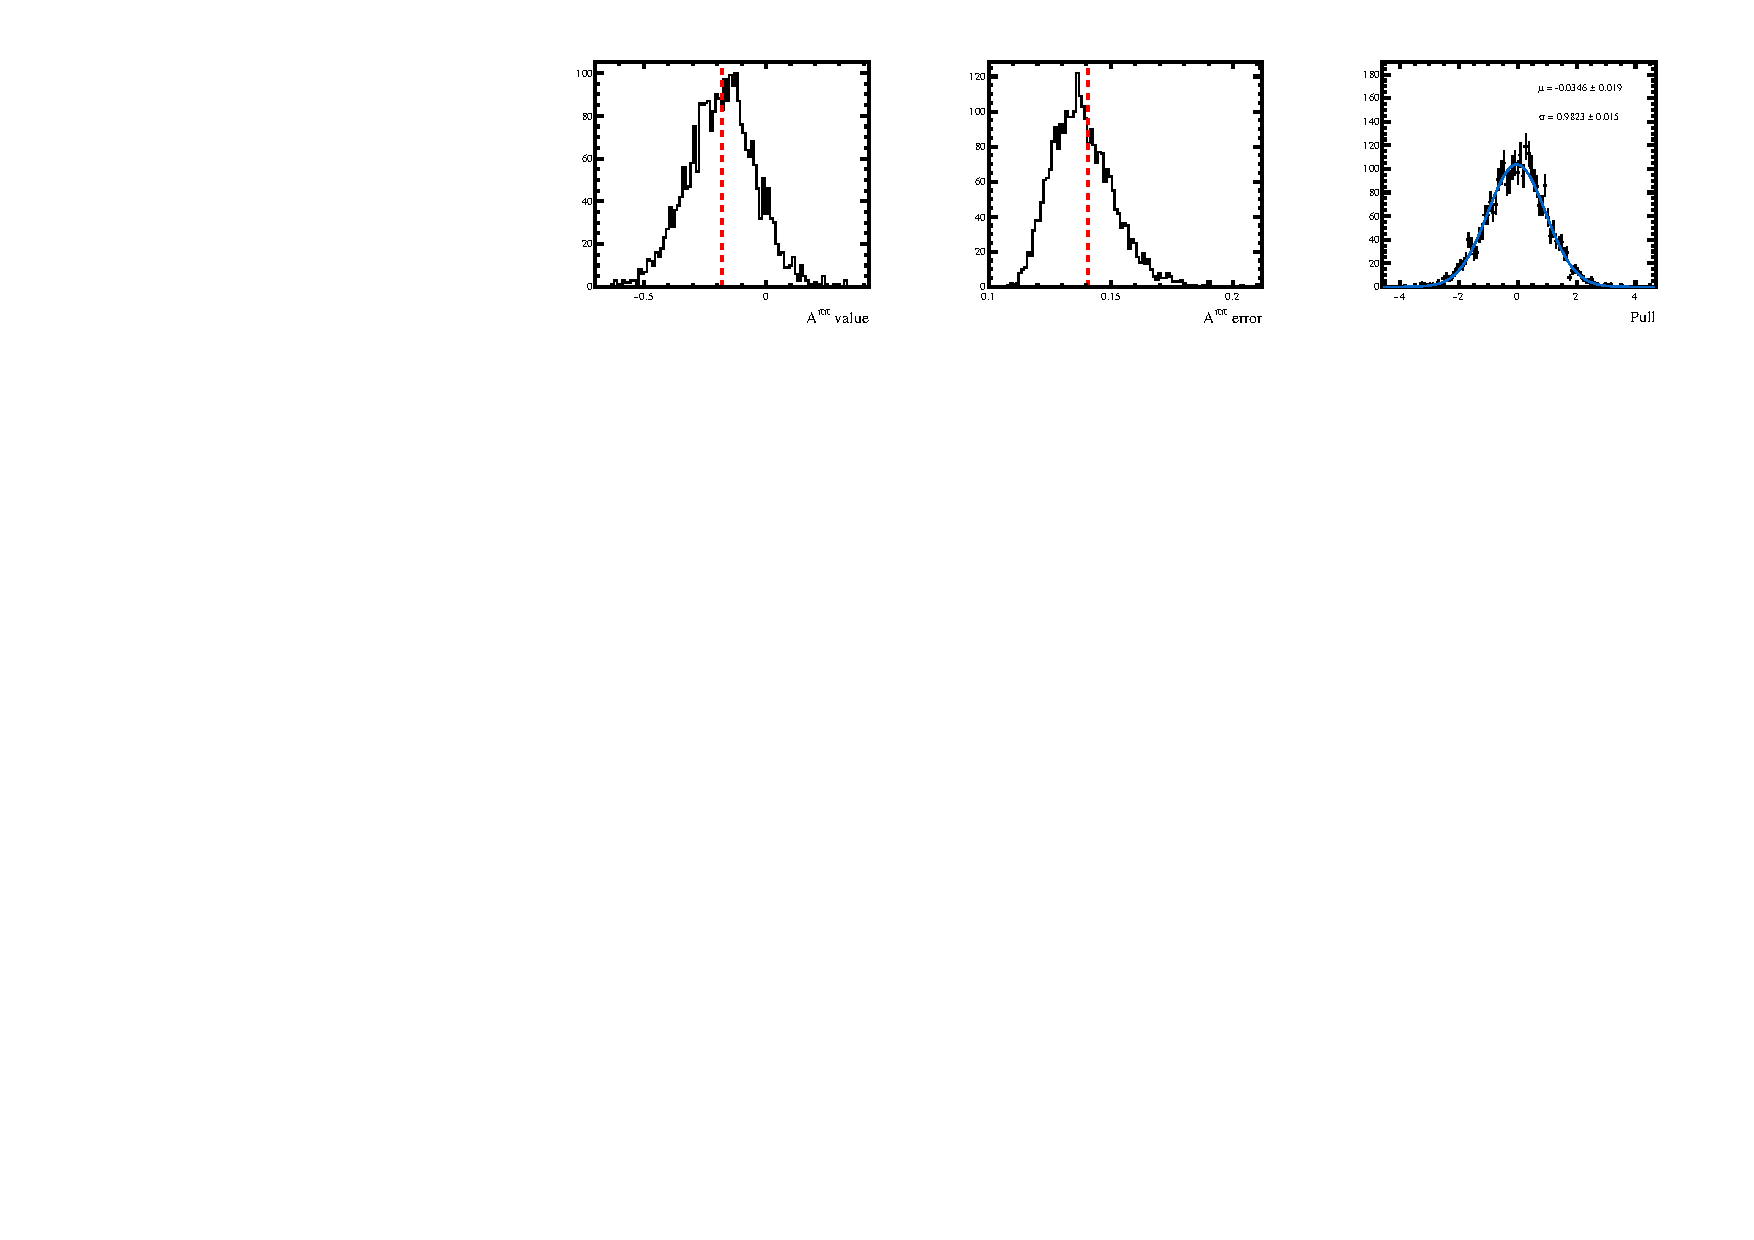
\includegraphics[width=\textwidth]{ANA_resources/Plots/Data_fit/FitterBias//CombinedRuns//A_signal_pipi.pdf} \\
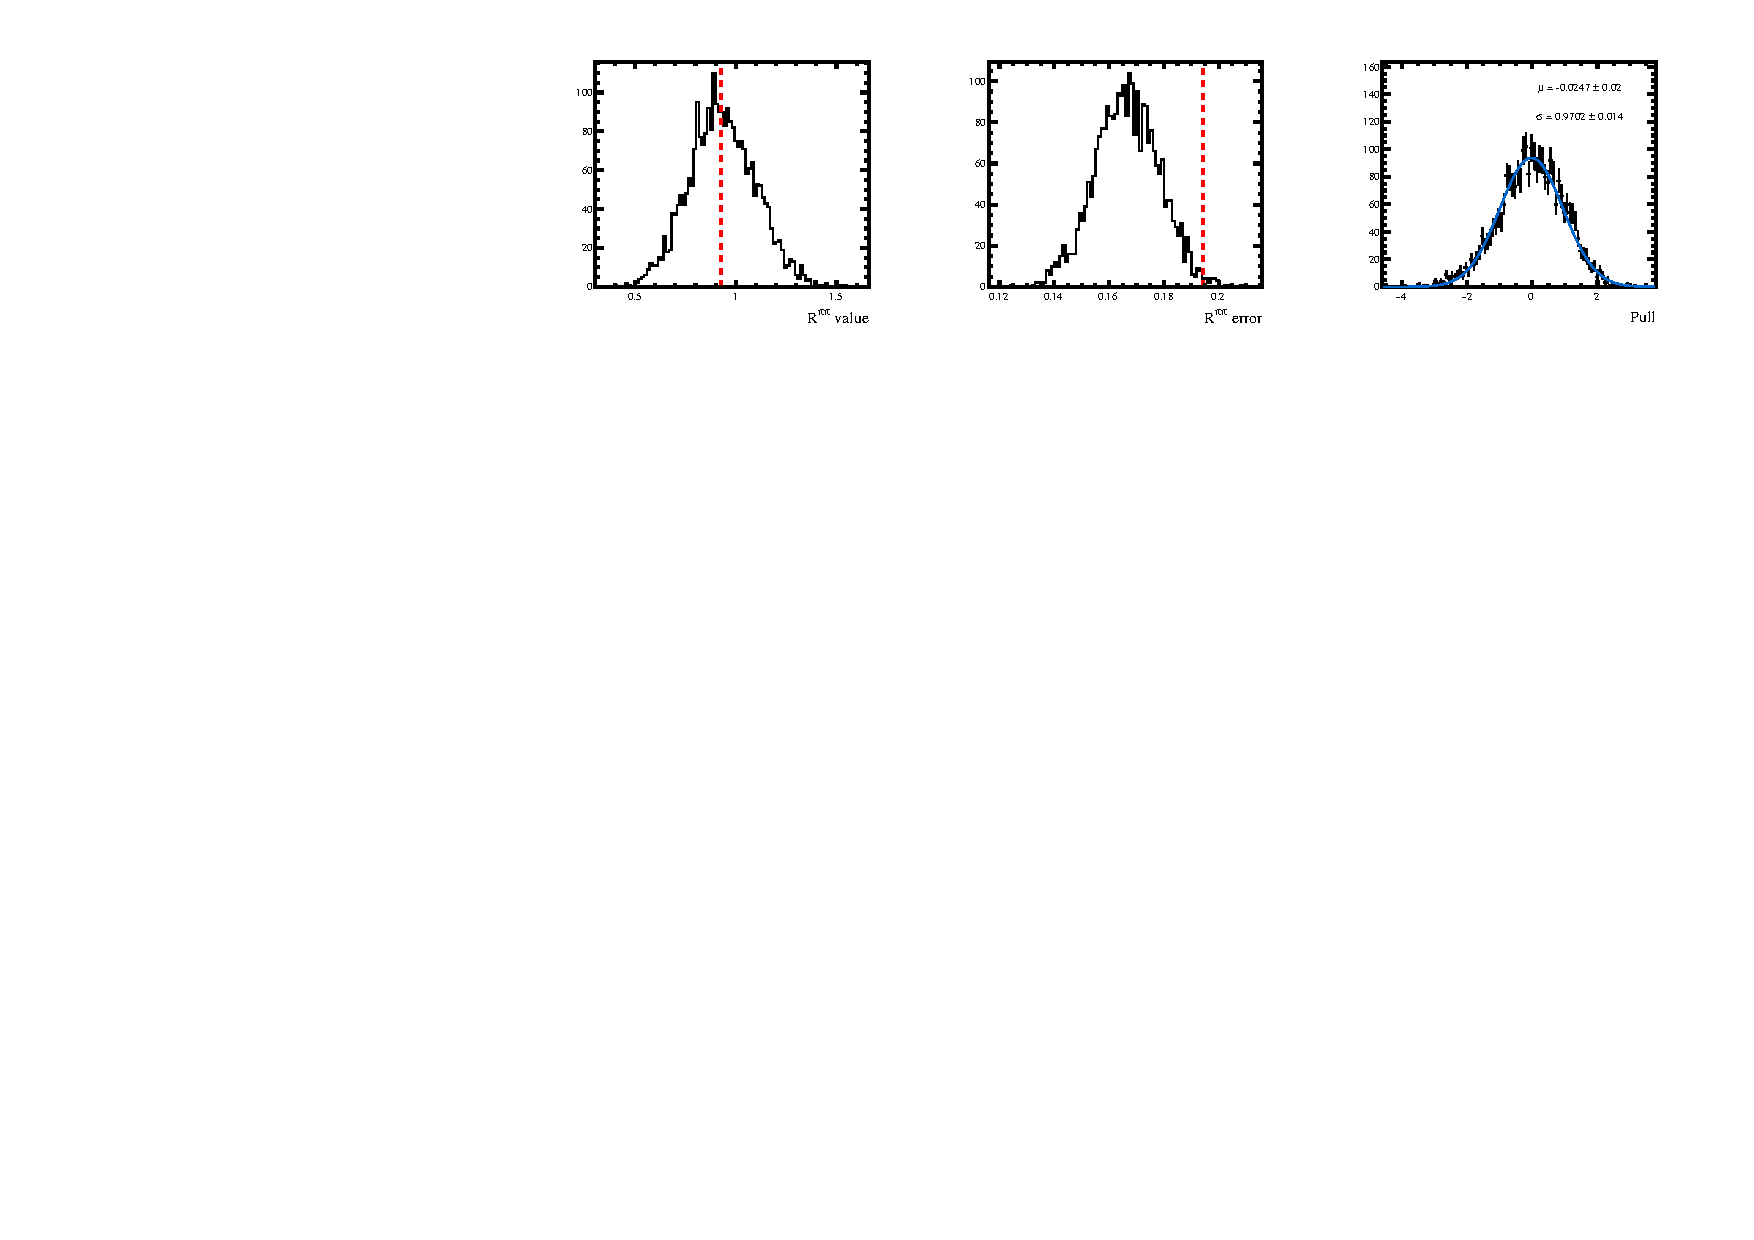
\includegraphics[width=\textwidth]{ANA_resources/Plots/Data_fit/FitterBias//CombinedRuns//R_signal_pipi.pdf} \\
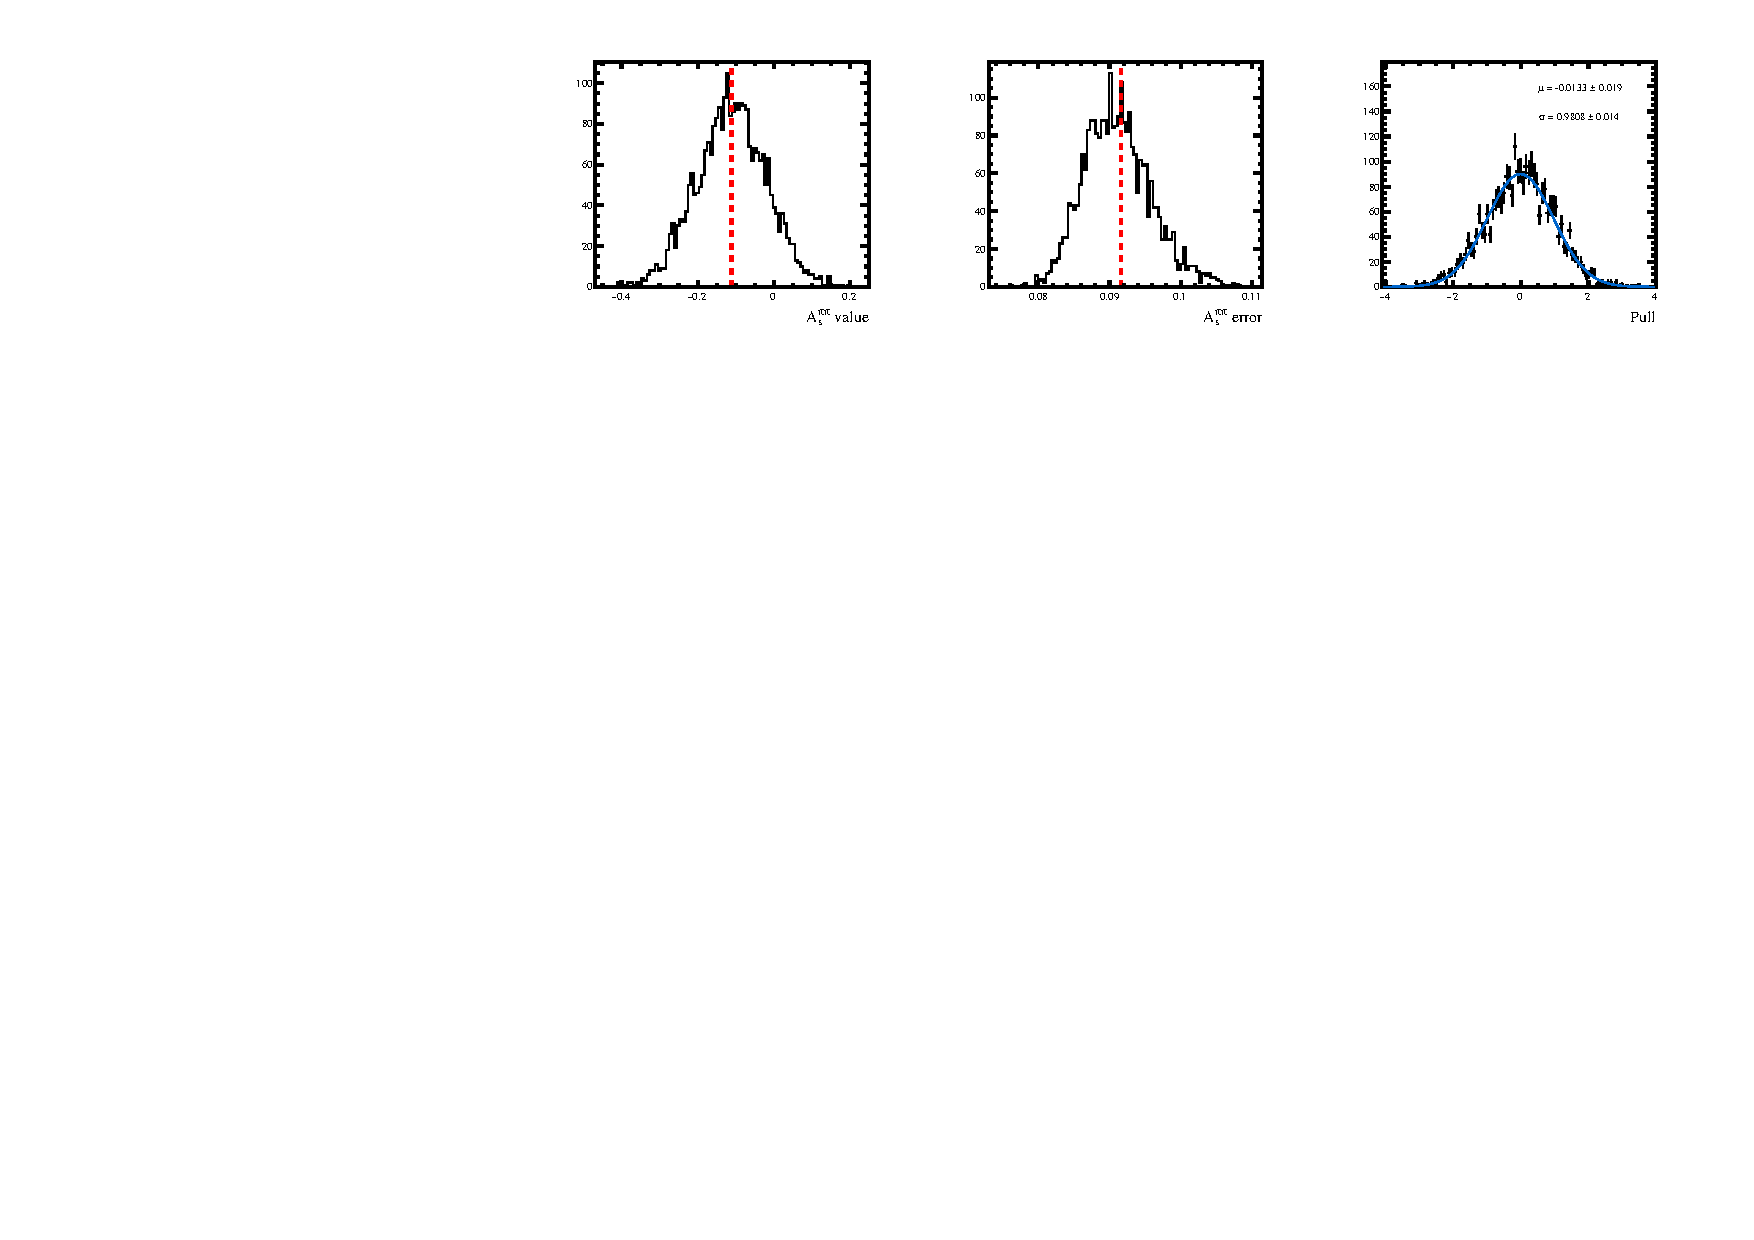
\includegraphics[width=\textwidth]{ANA_resources/Plots/Data_fit/FitterBias//CombinedRuns//A_Bs_pipi.pdf} \\
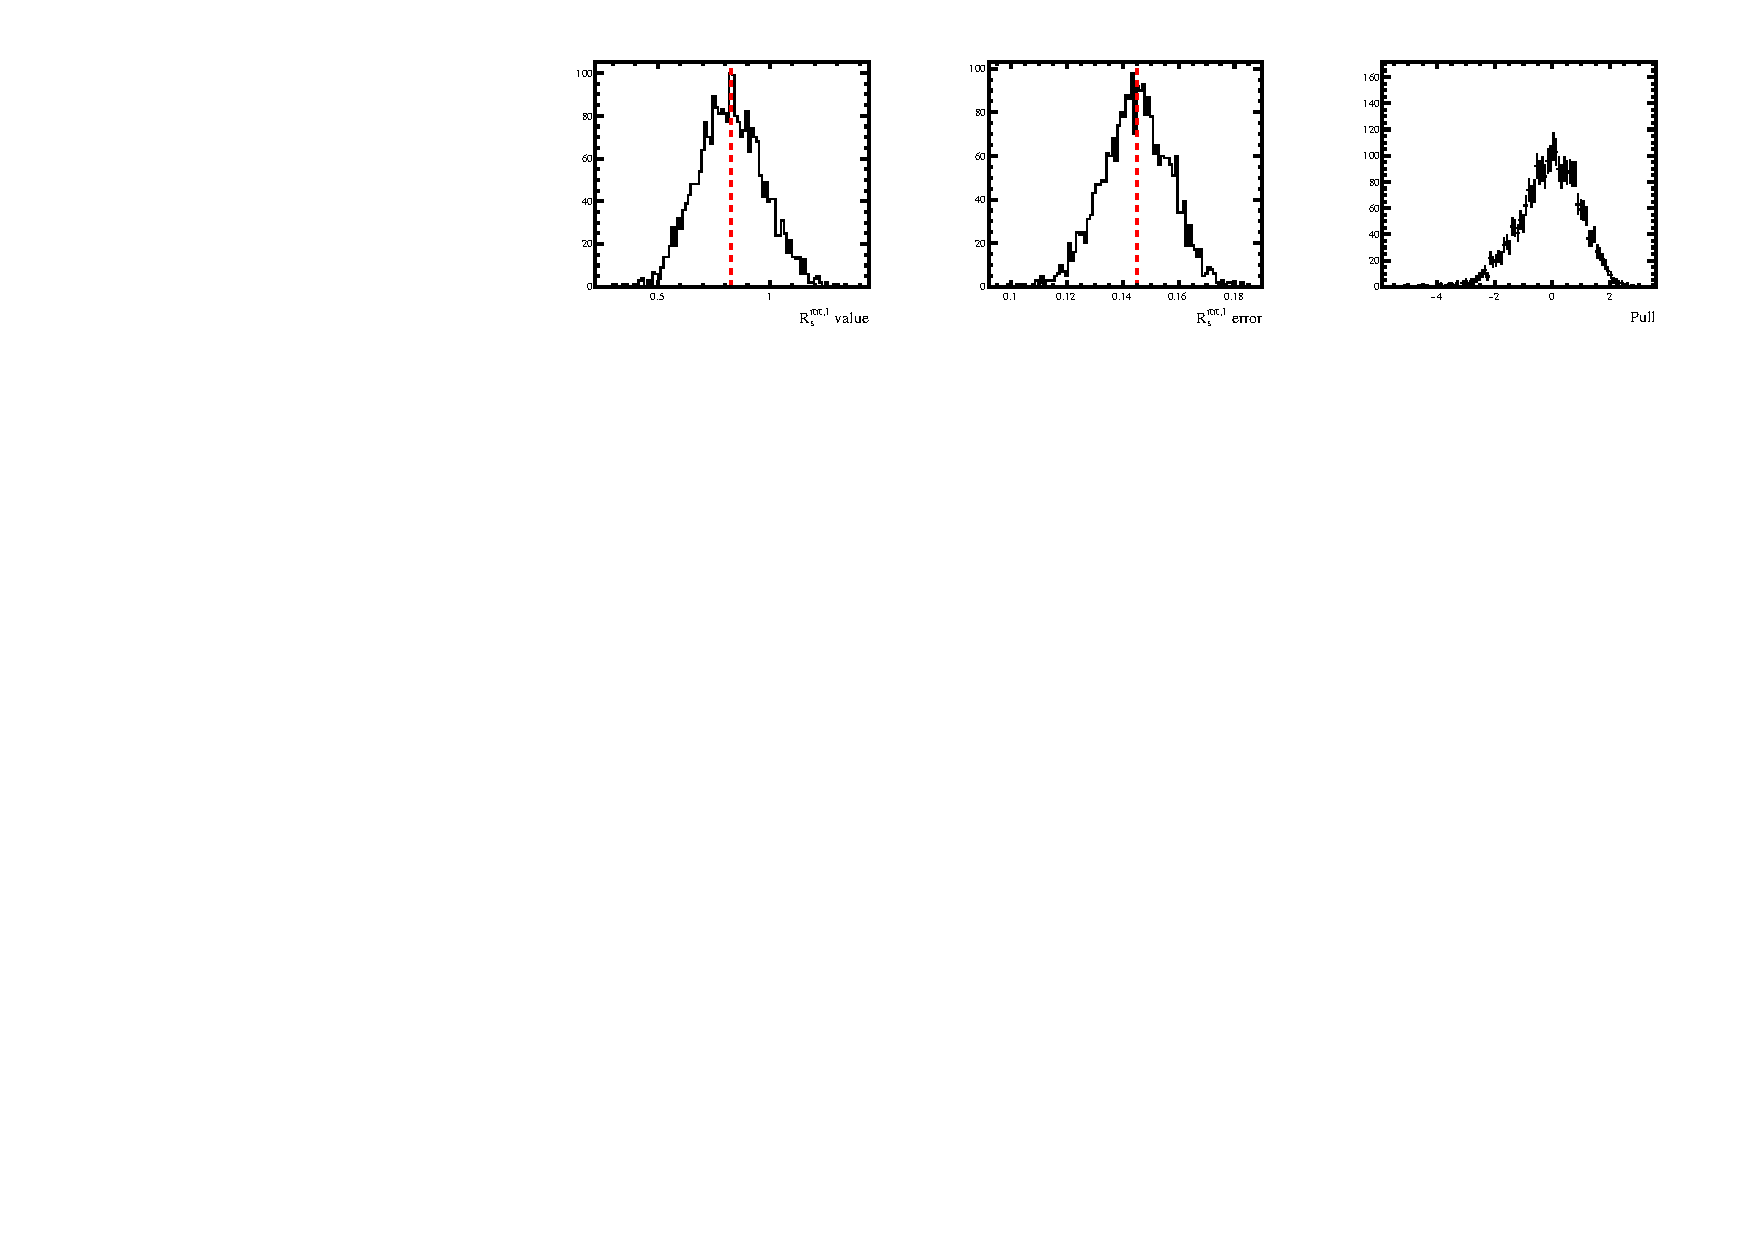
\includegraphics[width=\textwidth]{ANA_resources/Plots/Data_fit/FitterBias//CombinedRuns//R_Bs_pipi_run1.pdf} \\
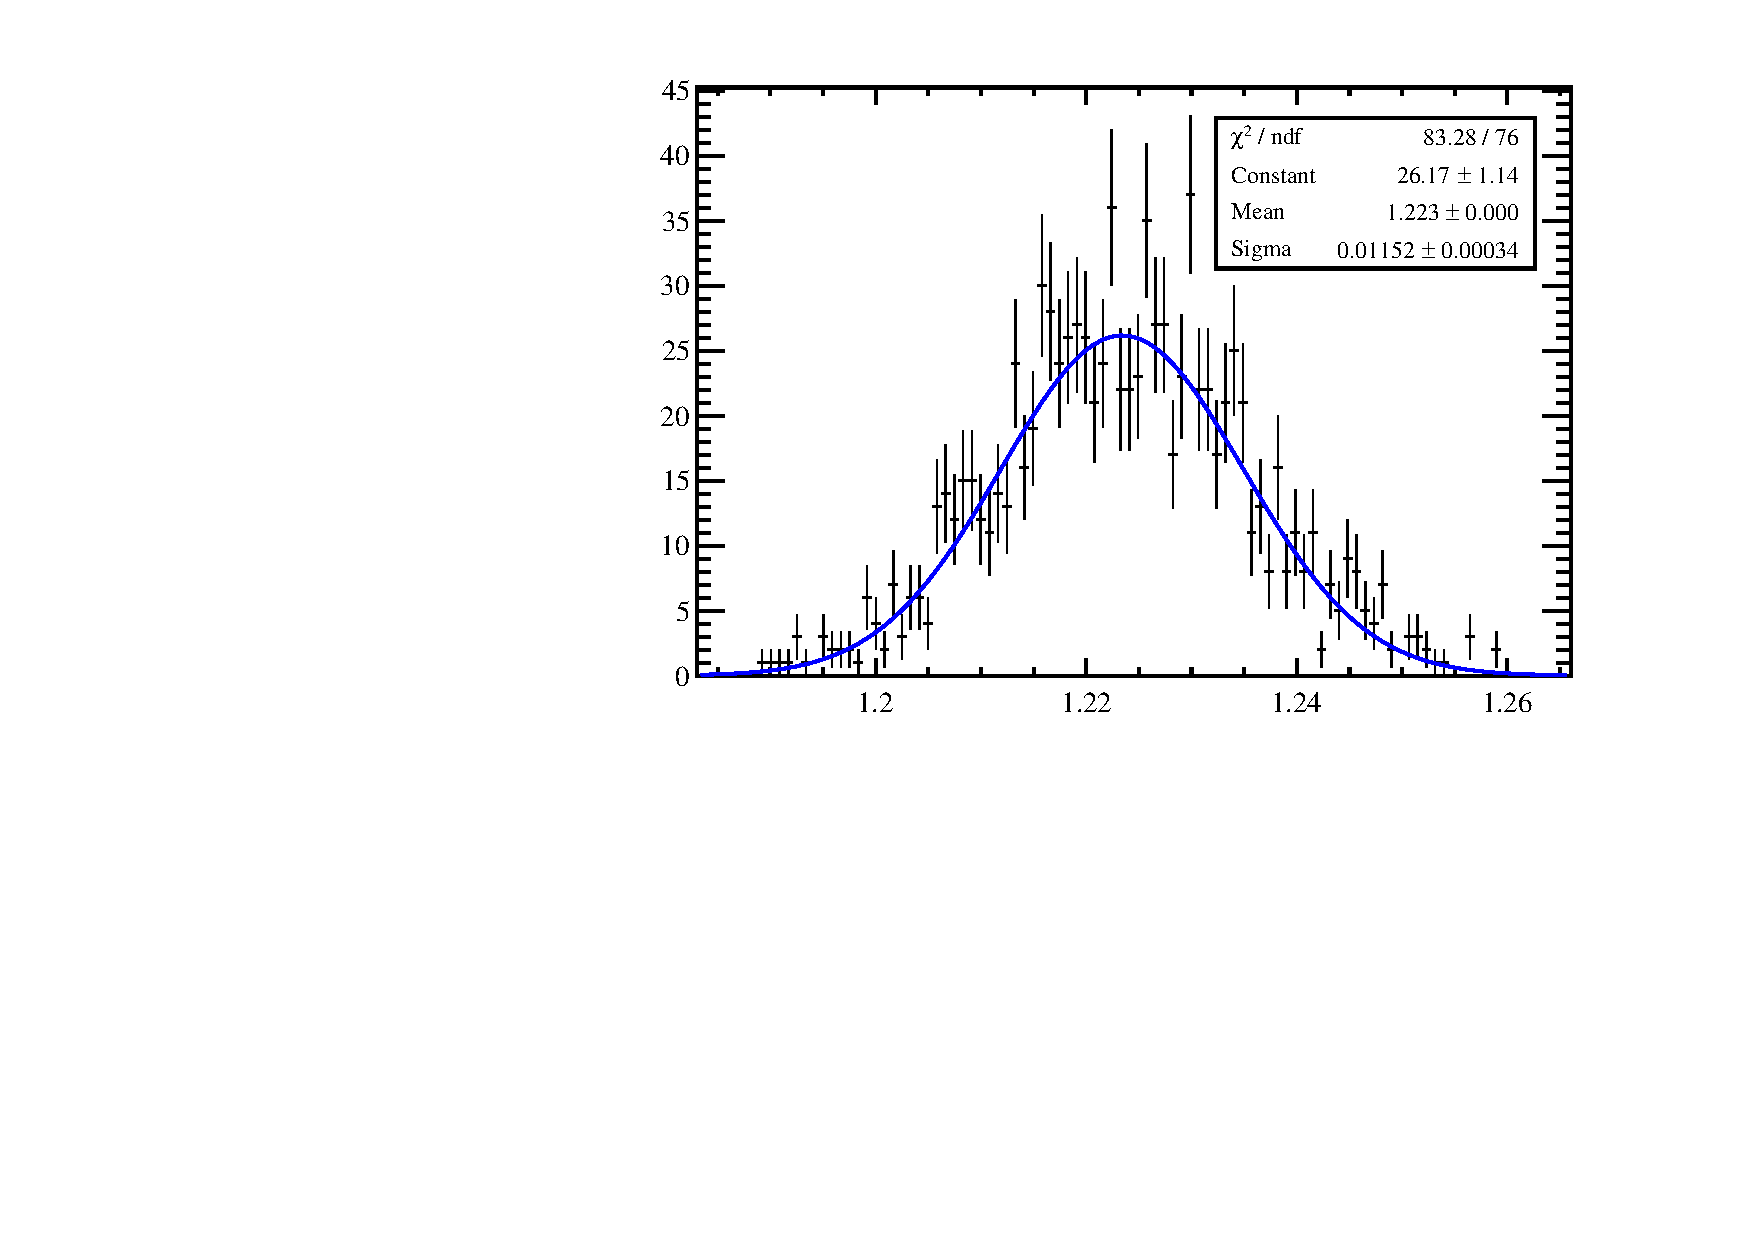
\includegraphics[width=\textwidth]{ANA_resources/Plots/Data_fit/FitterBias//CombinedRuns//R_Bs_pipi_run2.pdf} \\
  \end{tabular}
  \caption{Pull plots for $\pi\pi$ parameters of interest, obtained from generating and fitting 3000 toys using the data fit model. The left hand plot shows the fitted parameter distribution, with the value used to generate the parameter indicated with a dotted red line. The central plot shows the statistical uncertainty on the parameter obtained from the fit, with the statistical uncertainty of the parameter in the real fit to data indicated with a dotted red line. The right hand plot shows the pull distribution fitted with a Gaussian.}
\label{fig:pipi/CombinedRuns/_pulls}
\end{figure}
